\documentclass[a4paper,11pt]{article}
\usepackage[left=1cm, right=1cm, top=0.5cm, bottom=0.5cm]{geometry}
\usepackage{graphicx}
\usepackage{amssymb}
\usepackage{amsmath}
\usepackage{listings}
\usepackage{subfig}

\begin{document}

\section*{Phases and Magnitudes of $a_k$}


\begin{figure}[h]
    \centering
    \subfloat[Fourier series of $a$]{{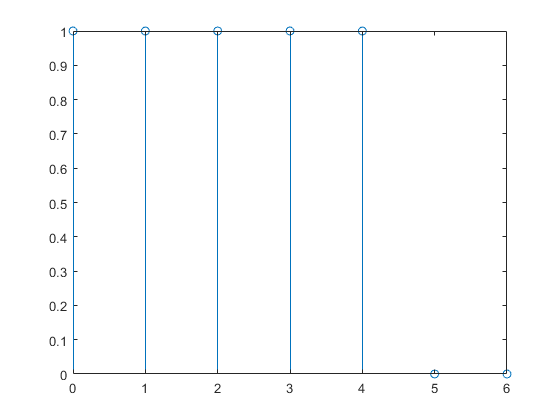
\includegraphics[width=7.5cm]{a_series.png} }}%
    \qquad
    \subfloat[Magnitude and Phase of $a$]{{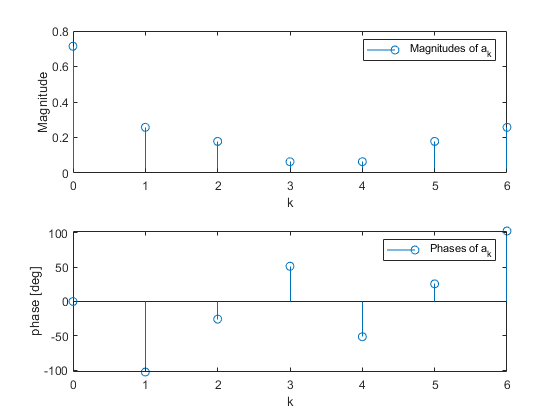
\includegraphics[width=7.5cm]{a_mag.png} }}%
    \caption{$3.28 (a)$}%
    \label{fig:example}%
\end{figure}

\begin{figure}[h]
    \centering
    \subfloat[Fourier series of $b$]{{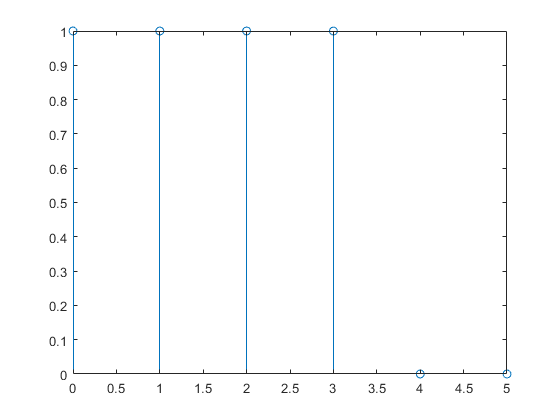
\includegraphics[width=7.5cm]{b_series.png} }}%
    \qquad
    \subfloat[Magnitude and Phase of $b$]{{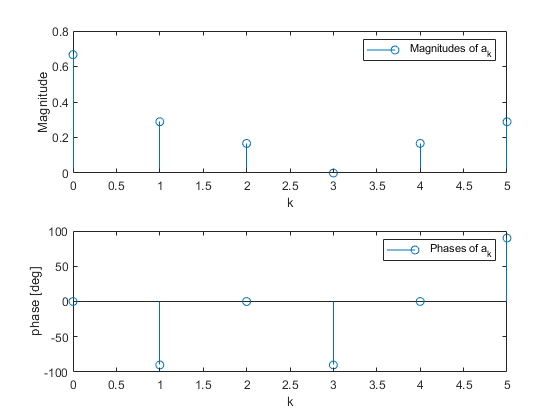
\includegraphics[width=7.5cm]{b_mag.png} }}%
    \caption{$3.28 (b)$}%
    \label{fig:example}%
\end{figure}

\begin{figure}[h]
    \centering
    \subfloat[Fourier series of $c$]{{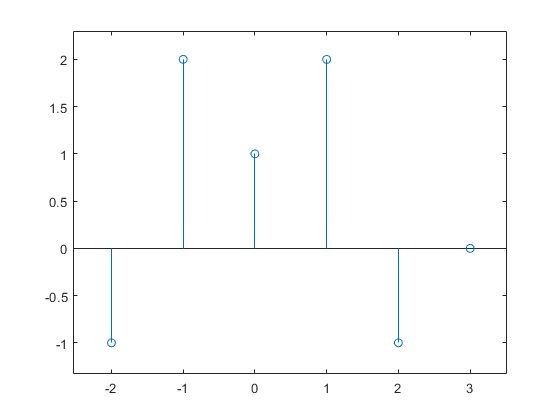
\includegraphics[width=7cm]{c_series.png} }}%
    \qquad
    \subfloat[Magnitude and Phase of $c$]{{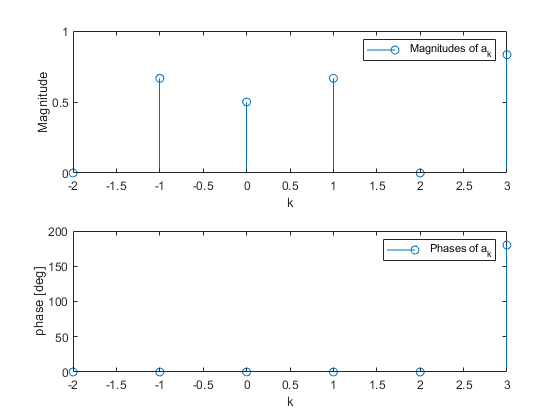
\includegraphics[width=7cm]{c_mag.png} }}%
    \caption{$3.28 (c)$}%
    \label{fig:example}%
\end{figure}
\end{document}